\chapter{Tests und Validierung}
\label{cha:testing}

\section*{Teststrategie}

Die Validierung der HydroNodeStation01 erfolgt in zwei Phasen: Zunächst auf dem Steckbrett-Prototyp mit dem Wio-E5 Mini Entwicklungsboard, anschließend auf dem Custom PCB nach dessen Lieferung von JLCPCB. Beide Phasen werden durch die Remote-Entwicklungsinfrastruktur unterstützt, die das Flashen, die serielle Konsole und eigene Analyse-Dashboards von beliebigen Standorten aus ermöglicht (s.\ Kapitel~\ref{cha:software}).

\section*{Tests mit dem Entwicklungsprototyp}

\subsection*{LoRaWAN-Konnektivität und Uplinks}

Der vollständige LoRaWAN-Uplink-Pfad wurde auf dem Wio-E5 Mini Entwicklungsboard erfolgreich verifiziert. Die Station verbindet sich zuverlässig über OTAA-Join mit dem Helium-Netzwerk und sendet reguläre Uplinks auf allen drei konfigurierten Ports (fPort 2, 3 und 4). Der eigene \textbf{SenseCAP M2 Helium-Miner} in der Entwicklerwohnung garantiert dabei perfekten Empfang auch im Innenbereich ohne externe Antenne, sodass Konnektivitätsprobleme als Fehlerquelle während der Entwicklung sicher ausgeschlossen werden können.

Im Feldtest wurde eine Reichweite von über \textbf{10~km} bei schwachem Signal nachgewiesen — weit über der für typische Einsatzszenarien im städtischen und ländlichen Raum benötigten Reichweite.

\subsection*{Sensor-Verifikation}

Alle sechs Sensoren wurden einzeln und im integrierten Betrieb auf Plausibilität und korrekte I2C-Kommunikation verifiziert:

\begin{itemize}
  \item \textbf{SHT45:} Temperatur- und Feuchtigkeitswerte konsistent und im erwarteten Bereich; Vergleich mit Referenzgerät zeigt gute Übereinstimmung.
  \item \textbf{BMP390:} Luftdruckwerte plausibel und stabil; Forced-Mode-Betrieb (Single-Shot + automatisches Sleep) verifiziert.
  \item \textbf{LTR390:} UV-Rohwerte reagieren korrekt auf UV-Exposition und zeigen erwartetes Verhalten bei Abdeckung des Sensors.
  \item \textbf{SCD41:} CO\textsubscript{2}-Single-Shot-Messungen liefern plausible Werte im typischen Innenraum-Bereich (400–1500~ppm). Das Pre-Measurement-Timing ist verifiziert: Die CO\textsubscript{2}-Messung ist stets fertig, wenn der Uplink-Zyklus beginnt.
  \item \textbf{SPS30:} Partikelmassenkonzentration und Zahlkonzentration reagieren korrekt auf Änderungen der Umgebungsluft (z.\,B.\ Zigarettenrauch-Exposition als Testfall). Fan-Cleaning-Mechanismus sowohl per Downlink-Befehl als auch automatisch nach 120~h verifiziert.
  \item \textbf{MAX17048:} Akkuspannungsmessung korrekt; batterie-adaptive Logik (Intervall-$\times2$ bei $< 3400\,\text{mV}$, Intervall-$\times12$ bei $< 3000\,\text{mV}$) im Testbetrieb verifiziert.
\end{itemize}

\subsection*{Downlink-Verifikation}

Beide Downlink-Befehle wurden erfolgreich getestet:

\begin{itemize}
  \item \textbf{0x11 — SPS30 Fan Cleaning:} Der SPS30 wird korrekt aufgeweckt, die Lüfterreinigung startet, der Cleanup-Timer stoppt den Sensor nach $10\,\text{s}$ automatisch und versetzt ihn in den Sleep-Modus.
  \item \textbf{0xFF — Software Reset:} Der STM32 führt einen sauberen Neustart durch; LoRaWAN-Join und periodische Uplinks werden korrekt aus dem NVM-Zustand wiederaufgenommen, ohne dass ein erneuter Join-Prozess nötig ist.
\end{itemize}

\subsection*{NVM-Persistenz}

Die Flash-basierte Persistenz des LoRaWAN-Zustands wurde durch mehrere absichtliche Neustarts verifiziert. In allen Fällen nahm die Station nach dem Neustart den Betrieb mit der bestehenden Session ohne erneuten Join wieder auf.

\subsection*{Strommessung am Prototyp}

Strommessungen mit dem PPK2 wurden am Steckbrett-Prototyp durchgeführt. Die Ergebnisse und deren Interpretation sind in Kapitel~\ref{cha:energie} vollständig dokumentiert. Der erhöhte Ruhestrom von ca.\ 3~mA wurde als prototyping-bedingt identifiziert und beeinträchtigt die Validität der Software und des Designs nicht.

\subsection*{I2C-Bus-Robustheit}

Der automatische I2C-Bus-Recovery-Mechanismus wurde durch absichtlich induzierte I2C-Fehler (Trennen und Wiederanschließen von Sensoren im Betrieb) verifiziert. In allen Fällen erkannte die Firmware den Fehler, führte den Bus-Recovery durch und setzte den Betrieb korrekt fort.

\newpage

\section*{Tests mit dem Custom PCB}
\label{sec:testing-pcb}

\subsection*{Elektrische Inspektion und Inbetriebnahme}

Nach Lieferung der Custom-PCBs von JLCPCB wurden visuelle Inspektion und erste elektrische Verifikationen durchgeführt. Dabei wurde ein Fehler im TPS63900-Spannungsregler identifiziert (s.\ Kapitel~\ref{cha:probleme} und~\ref{sec:pcb-review}). Mit dem beschriebenen Breakout-Workaround läuft das PCB stabil.

\subsection*{Sensor-Verifikation auf dem Custom PCB}

Alle fünf Kernsensoren wurden auf dem Custom PCB erfolgreich verifiziert:

\begin{itemize}
  \item \textbf{SHT45:} Temperatur- und Feuchtigkeitswerte plausibel und stabil im Außenbetrieb.
  \item \textbf{BMP390:} Luftdruckwerte korrekt; Forced-Mode-Betrieb auf dem Custom PCB verifiziert.
  \item \textbf{LTR390:} UV-Index wird korrekt berechnet und kalibriert. UV-Rohwerte reagieren auf UV-Exposition. Die Berechnung wurde während des Projekts refaktoriert, sodass der Sensor direkt den UV-Index (UVI) ausgibt. Der Einfluss der Acrylglas-Abdeckung des Stevenson-Screen-Gehäuses wurde empirisch ermittelt: Messwerte mit und ohne Glas unter direkter Sonneneinstrahlung ergaben ein Verhältnis von $6{,}8 / 5{,}2 = 17/13$, das als ganzzahliger Korrekturfaktor in der Firmware angewandt wird (s.\ Abschnitt Hardware: UV-Sensorschutz).
  \item \textbf{SCD41:} CO${}_2$-Messungen plausibel im Außenbereich (ca.\ 400~ppm). Pre-Measurement-Timing verifiziert.
  \item \textbf{SPS30:} Partikelmassenkonzentration und Zahlkonzentration reagieren korrekt auf Umgebungsluft.
\end{itemize}

\subsection*{LoRaWAN und Netzwerk}

Die Station verbindet sich zuverlässig über OTAA-Join mit dem Helium-Netzwerk und sendet reguläre Uplinks auf allen drei konfigurierten Ports (fPort 2, 3 und 4). LoRaWAN-Daten fließen über Amazon SNS in das HydroNode-Backend und sind in Echtzeit auf dem öffentlichen Dashboard einsehbar.

\subsection*{Strommessung (PPK2)}

Strommessungen mit dem Nordic Semiconductor Power Profiler Kit II (PPK2) wurden am Custom PCB durchgeführt. Die Messdatei (\texttt{ppk2-20260601T143444.ppk2}) enthält Aufnahmen des STOP2-Ruhestroms sowie der TX-Spitzenströme. Ergebnisse und Interpretation sind in Kapitel~\ref{cha:energie} dokumentiert.

\subsection*{Langzeit-Feldtest}

Die Station befindet sich seit Ende Mai 2026 im Außeneinsatz im selbst entworfenen Stevenson-Screen-Gehäuse aus ASA. Der Feldtest läuft ohne Unterbrechungen. Alle Sensoren liefern kontinuierlich stabile Werte; der LoRaWAN-Uplink ist zuverlässig aktiv. Echtzeit-Messwerte und Verlaufsdaten sind öffentlich einsehbar unter:\\
\url{https://hydronode.texhfexlabs.de/stations/public/004dd7e7-5c27-4de0-bff5-24116f721658}

\begin{figure}[H]
  \centering
  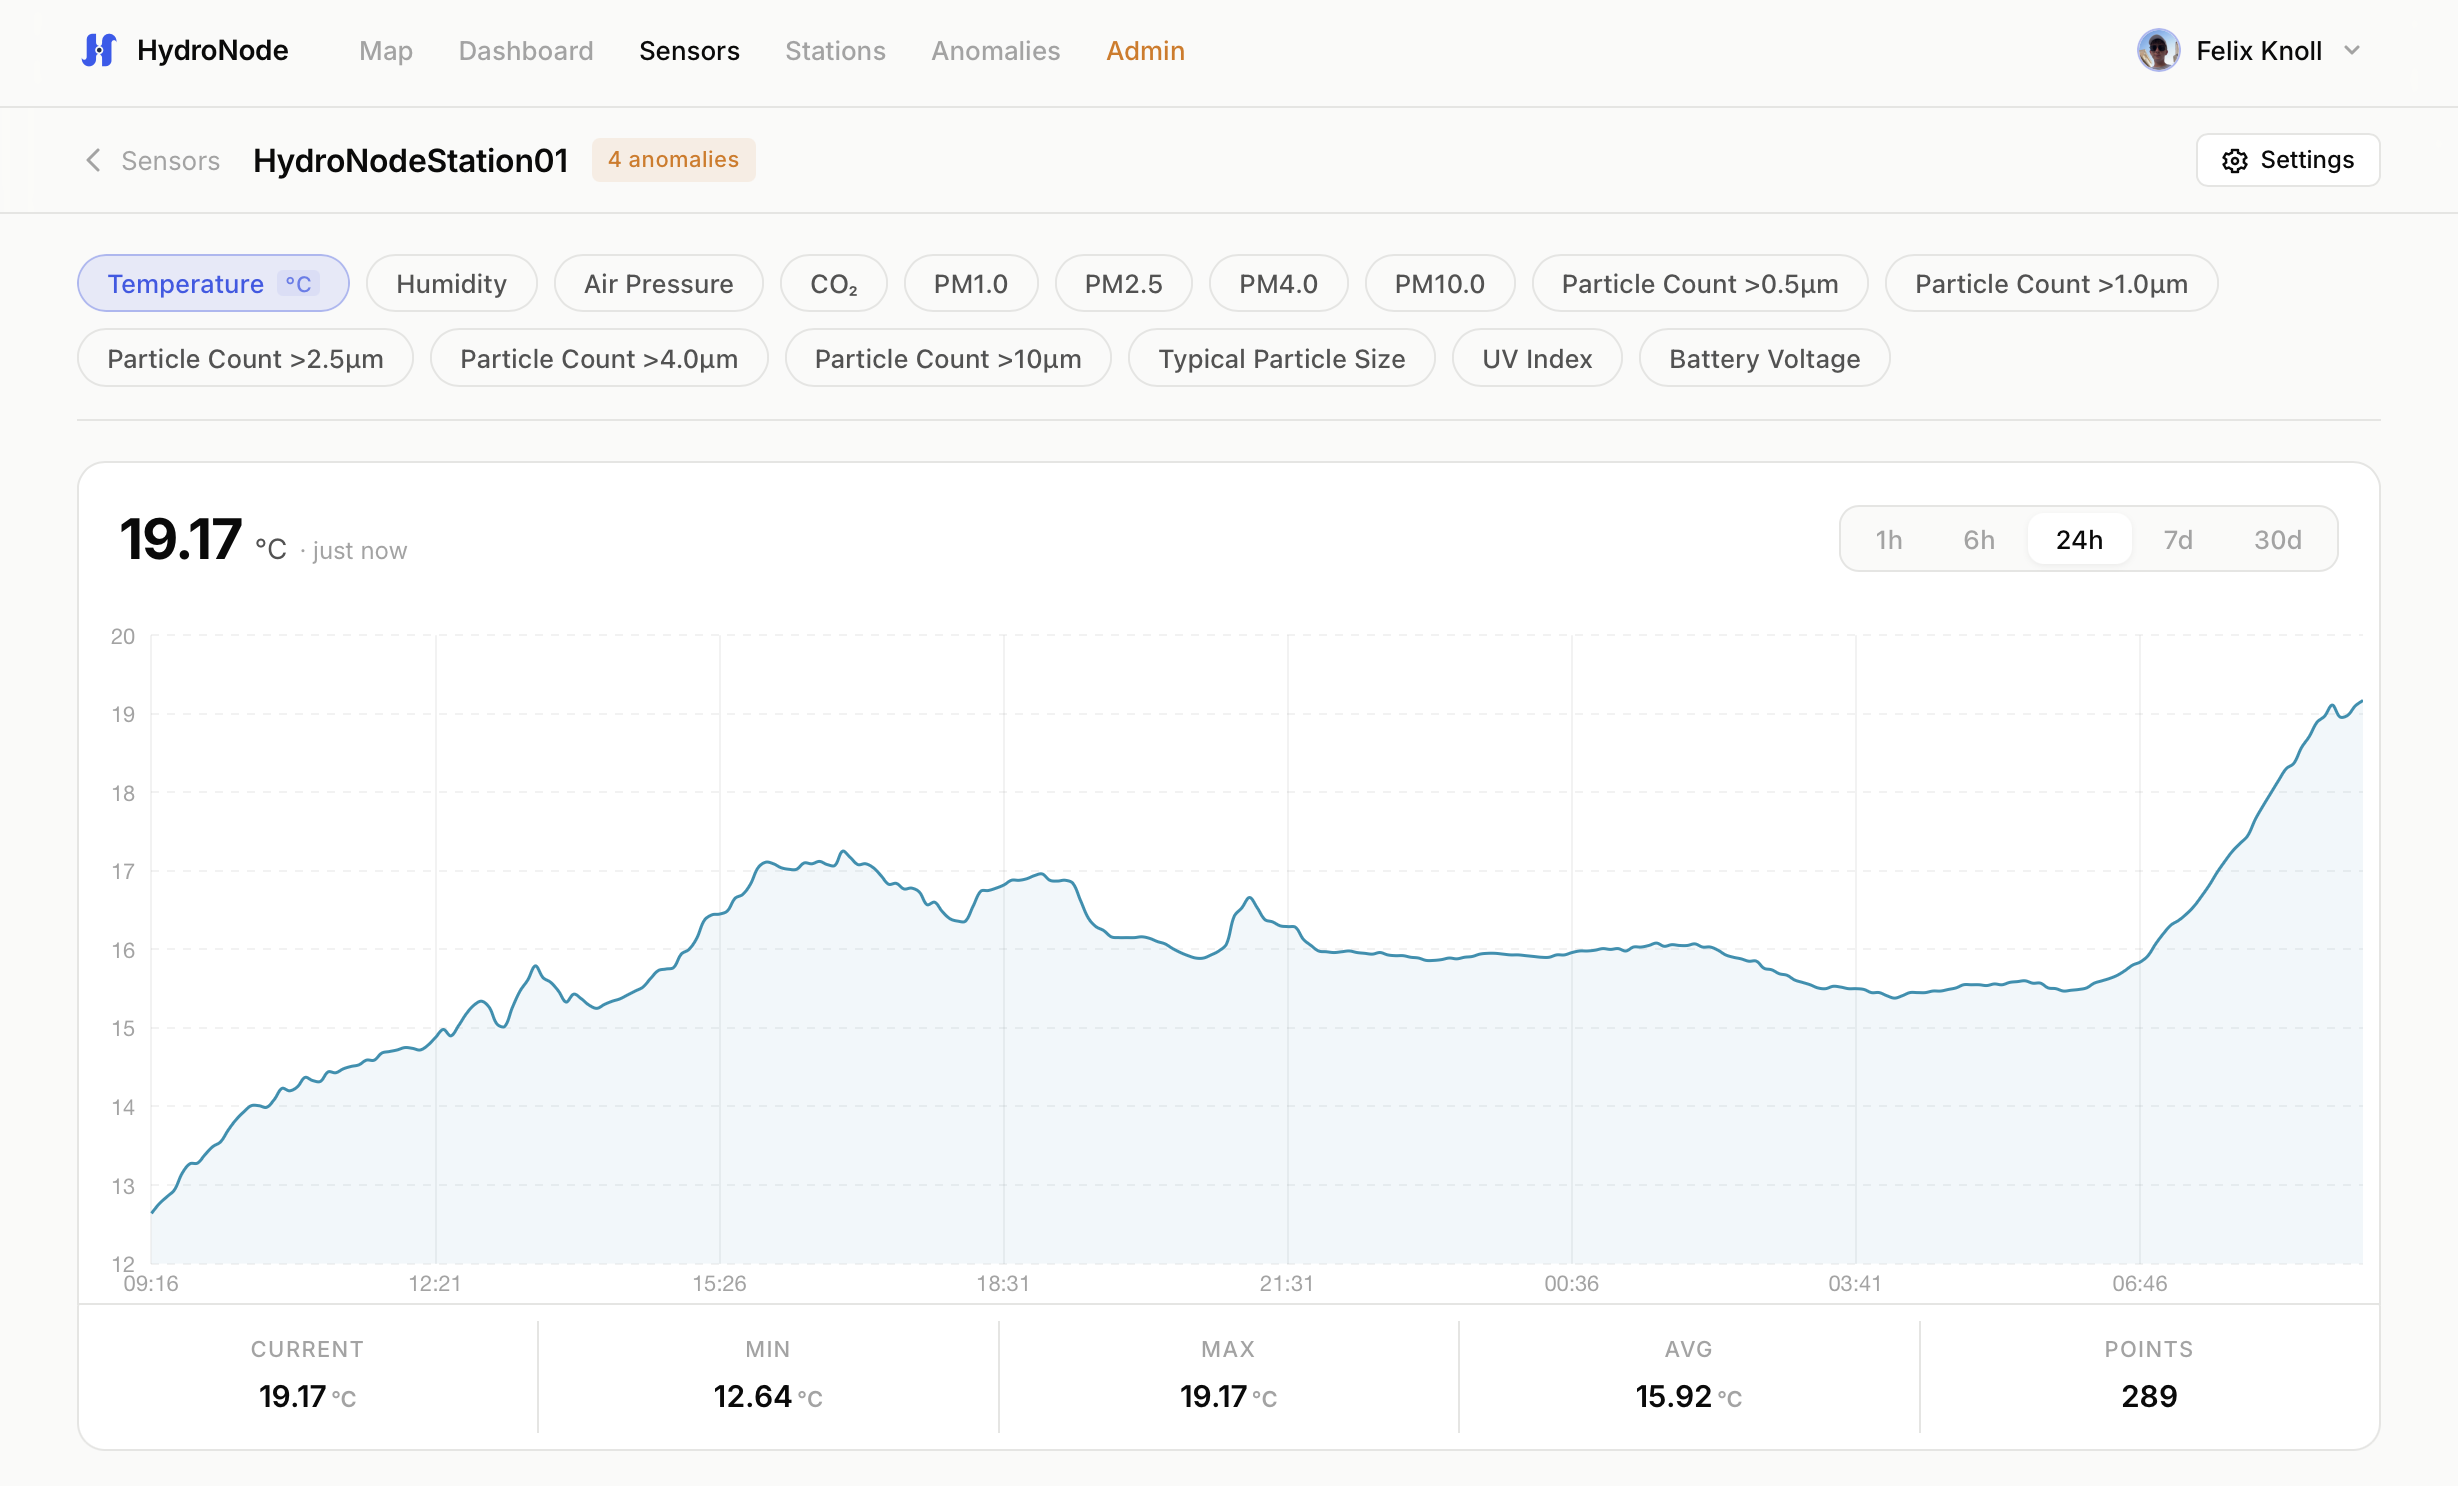
\includegraphics[width=\linewidth]{../assets/dashboard_preview}
  \caption{Live-Dashboard der HydroNodeStation01 mit Feldtest-Messdaten}
  \label{fig:dashboard-fieldtest}
\end{figure}

\subsection*{Noch ausstehend}

\begin{itemize}
  \item \textbf{Solar-Verifikation:} Prüfung der Solar-Ladefunktion (BQ25185) unter verschiedenen Lichtbedingungen, insbesondere an bewölkten Tagen.
  \item \textbf{Langzeit-Batterielaufzeit:} Vergleich gemessener vs.\ theoretisch berechneter mittlerer Strom über einen vollständigen Entladezyklus.
\end{itemize}
